\documentclass[titlepage,11pt,a4paper]{article}
\usepackage{xunicode}
\usepackage{fontspec}
\usepackage[frenchb]{babel}
\usepackage[hidelinks]{hyperref}
\usepackage{multirow}
\usepackage{array}
\usepackage{adjustbox}
\usepackage{tabu}
\usepackage{booktabs}
\usepackage{moresize}
\usepackage{graphicx}
\usepackage{titlepic}

\setmainfont[Ligatures=TeX]{Linux Libertine O}

\setlength\extrarowheight{3pt}

\title{Bilan de formation BAFD}
\author{Julien Durillon\\Dossier 837177-XURK\\9 rue de Chypre\\44000 NANTES}

\titlepic{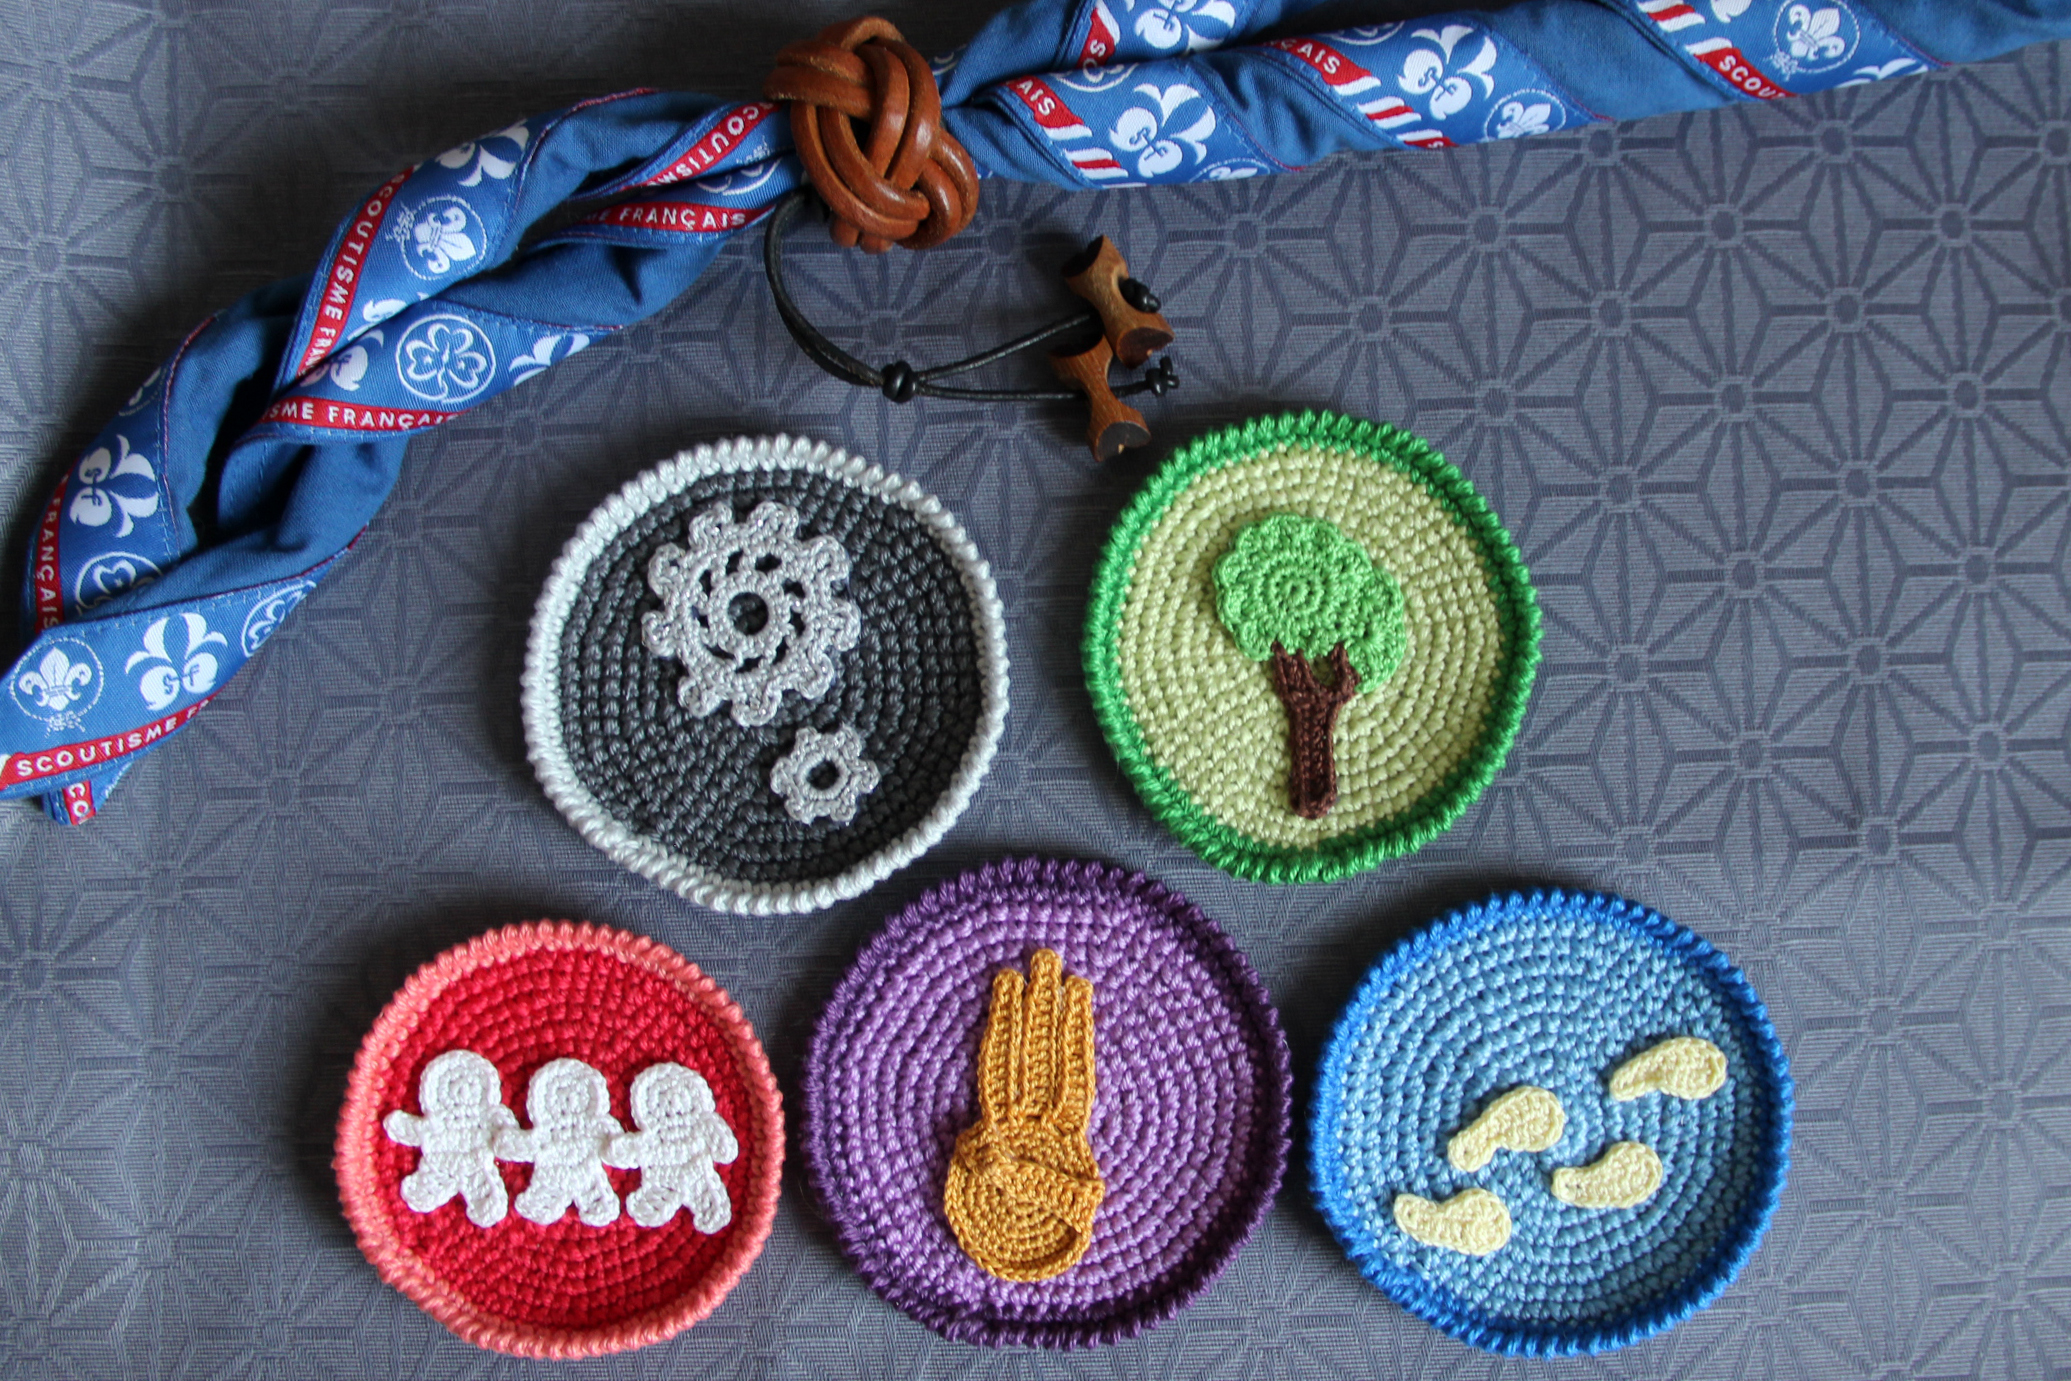
\includegraphics[width=\textwidth]{./foulard-rondelles.jpg}}

\parskip1.3mm

\begin{document}

\maketitle

\tableofcontents

\clearpage

\section{Mon parcours d'animateur à directeur}

\subsection{Mon engagement dans le scoutisme}

J'ai commencé mon parcours scout en 1998 dans l'association ``Scouts de France'' puis ``Scouts et Guides
de France'' (identifiée dans ce bilan sous le sigle SGDF). Commencé à 8 ans, cet engagement dans le scoutisme
m'a guidé vers un rôle d'animateur à partir de 2009.

J'ai endossé ce rôle d'animateur en premier lieu pour rendre bénévolement au mouvement ce
qu'il m'avait apporté, en participant à l'éducation de jeunes. Puis les
formations BAFA que j'ai suivies chez les SGDF, et notamment l'approfondissement, m'ont
permis de me familiariser avec le projet éducatif de l'association. Ce faisant, mon
engagement est passé d'un simple «\,rendre aux suivants ce que j'ai reçu\,» à une
appropriation du projet éducatif de l'association.

J'ai été animateur bénévole SGDF pendant cinq ans dont deux ans en tant que directeur
d'accueil de scoutisme. Pour ces deux dernières années, j'étais qualifié Directeur du Scoutisme Français.

Pendant ces années d'animation, j'ai pu découvrir le projet éducatif des
Scouts et Guides de France. J'ai pu apprendre à me positionner par rapport au projet
éducatif et à construire des projets pédagogiques répondant à ce dernier et aux besoins
des jeunes. J'ai pu expérimenter plusieurs postes: responsable sanitaire,
responsable de l'intendance, de l'économat et enfin directeur d'accueil de scoutisme.

\subsection{Une volonté de me former et de former}

Au terme de ces cinq années d'animation, j'ai accepté une mission d’accompagnateur pédagogique.
Mon rôle était d'accompagner les équipes d'animateurs sur mon département à la réalisation
d'activités et à la construction de projets pendant l'année et pour les camps d'été.
Je me suis également retrouvé dans le rôle de formateur. Et en tant que tel, j'avais le
devoir d'aller me former moi-même à cette nouvelle mission.

En parallèle de cette envie de me former pour être plus à l'aise dans mon rôle,
j'ai été appelé à m'inscrire en cursus BAFD\@. En particulier pour assurer par la suite la
direction de stage de formation BAFA\@. De plus, ma mission m'amènera à organiser et
diriger des camps accompagnés.  J'envisage également de me forger une expérience de formateur dans d'autres organismes de
formation BAFA\@.

Un camp accompagné, chez les SGDF, est un accueil de scoutisme déclaré par l'échelon
départemental ou national. Il propose à des groupes de jeunes et leurs animateurs
ne possédant pas de directeur de vivre des camps scouts. Cette structure permet à
des animateurs stagiaires de se former pendant leurs camps. L'équipe de direction accompagne les différents
camps installés sur le lieu de l'accueil. Les qualifications du scoutisme français
permettent d'organiser et de diriger un tel accueil sans BAFD\@. Personnellement, je
juge qu'au dessus d'un certain nombre de jeunes encadrés, il est nécessaire pour un
directeur d'avoir un certain bagage. Notamment le recul sur la
direction que peut apporter la formation BAFD\@.

\subsection{Mon projet de initial de formation}

Au début de mon cursus BAFD, en arrivant à la formation générale, j'avais déjà dirigé deux
accueils de scoutisme.

J'avais expérimenté la fonction de directeur d'accueil de scoutisme:
prendre en charge les tâches administratives; travailler avec et diriger une équipe d'animateurs;
construire les projets pédagogiques de chaque accueil. J'ai également eu à accompagner des
stagiaires BAFA pendant les accueils de scoutisme que j'ai dirigés avant de commencer ma
formation BAFD\@.

La session de formation générale m'a permis de prendre du recul sur mes pratiques, de
faire le point sur mon parcours de formation et d'évaluer mon positionnement par rapport
aux fonctions du directeur d'accueil collectif de mineurs.

\subsubsection{Mes atouts}

En début de parcours, mes points forts résidaient dans:

\begin{itemize}
   \item La construction et le suivi d'un projet pédagogique prenant en compte le
      projet éducatif de la structure ainsi que les besoins des jeunes;
   \item La prise de décision, la transmission de consigne, la répartition de la charge;
   \item La gestion de la vie quotidienne d'un accueil de scoutisme;
   \item La communication auprès des familles des jeunes, avant, pendant et après le
      séjour;
   \item La capacité à assurer la sécurité physique et affective des enfants et des
      jeunes.
\end{itemize}

En cette fin de parcours de formation, je reconnais que j'étais surtout à l'aise dans
l'animation d'une équipe de personnes que j'ai appris à connaître pendant l'année,
en phase avec mes convictions, dans une relation de confiance construite sur plusieurs mois.

\subsubsection{Les axes d'amélioration}

Pendant mon parcours de formation, j'ai pu déterminer les axes d'amélioration suivants:

\paragraph{La gestion financière de d'accueil} En effet, je n'en avais
qu'une seule expérience avant de commencer mon parcours de formation. J'ai fait de cette
expérience un bilan mitigé. J'ai donc identifié ce point comme un axe d'amélioration.

\paragraph{Le suivi administratif de l'accueil au quotidien} Étant épaulé par des
personnes ressources de mon association, j'ai très peu eu l'occasion de gérer le suivi
administratif pendant mes accueils.

\paragraph{L'accompagnement d'un adulte en formation} J'ai eu l'occasion d'accompagner un
stagiaire BAFA avant de commencer mon parcours BAFD\@. Je jugeais néanmoins que cet
accompagnement était insuffisant. De mon point de vue, je manquais d'expérience dans ce
domaine.

\label{analysepersonnelle}
\paragraph{La communication au sein de l'équipe d'animation} J'ai vécu ce manque lors du
dernier accueil que j'ai dirigé avant de débuter ma formation. J'avais cinq animateurs avec moi,
globalement peu formés. Les quotas d'encadrement étaient respectés, mais les conditions
n'était pas confortables. J'ai expérimenté le manque de communication dans l'équipe et ses
effets néfastes sur l'ambiance et l'organisation de l'accueil.

\paragraph{La mise en place de partenariats dans le cadre de l'accueil} Au début de ma
formation je n'avais eu que très peu d'occasions de développer des partenariats. Les
projets menés avec les jeunes ne m'ont amené qu'une seule fois à construire un
partenariat.

\paragraph{La connaissance d'une autre association et d'un autre projet éducatif} Ayant
été jeune, animateur puis directeur SGDF, je n'ai pas eu l'occasion de découvrir d'autres
modes d'accueils collectifs de mineurs. Il me semblait important de me confronter à
d'autres types d'accueils.

\paragraph{Le recrutement d'un animateur} Le recrutement est traditionnellement délégué à
des personnes ressources parmi les parents des jeunes. Avant de commencer ma formation, je
n'ai pas eu l'occasion de recruter un animateur pour un accueil que je dirigeais.

\paragraph{} J'ai donc construit mon parcours de formation pour répondre à ces axes d'amélioration.


\clearpage
\section{Chronologie de mon cursus}

Toutes les étapes de mon parcours se sont déroulées au sein des Scouts et Guides de
France, avec une nuance sur mon deuxième stage pratique.

J'ai effectué ma formation dans cette association pour trois raisons. Premièrement,
les sessions de formation ajoutent au cahier des charges BAFD des éléments utiles dans ma
mission actuelle. Deuxièmement, je n'ai pas trouvé de premier stage de direction dans les ACM qui
m'intéressaient. Mes disponibilités n'étaient pas compatibles avec leurs besoins. Néanmoins,
mon deuxième stage pratique m'a amené à sortir de ma zone de confort et de mon association
de référence.

L'association «\,Scouts et Guides de France\,» fait partie des 9 associations de scoutisme agréées par
l'état et par conséquent organise des «\,accueils de scoutisme\,» tels que définis par
l'article 227--1 du code de l'action sociale et des familles. Le but des SGDF est d'éduquer
des enfants et des jeunes et les inviter à être des citoyens heureux, utiles, actifs et artisans
de paix. Pour ce faire, les SGDF proposent d'utiliser la méthode scoute, présentée en
annexe, page~\pageref{methsc}.

Pour se donner les moyens de faire vivre la méthode scoute aux enfants et aux jeunes, les
Scouts et Guides de France sont organisme de formation BAFA et BAFD\@. En plus de répondre aux cahiers des
charges du BAFA et du BAFD, les formations SGDF contiennent des volets répondant aux objectifs
de formation des responsables du mouvement. Ces formations se basent notamment sur cette même méthode scoute.

\subsection{Session générale}

J'ai effectué ma session générale chez les SGDF en avril 2014.
Outre la réalisation du cahier des charges de la formation générale BAFD,
cette formation propose aux stagiaires de creuser les origines de la méthode scoute. Ces
derniers sont également invités à questionner la pédagogie mise en place par les SGDF\@.
Cette session propose deux volets: le développement du scoutisme et l'accompagnement des bénévoles.

J'ai choisi le parcours «\,accompagnement\,». Cela m'a permis de prendre du recul sur mes
pratiques et d'obtenir des connaissances théoriques utiles pour ma mission
d’accompagnateur pédagogique pendant l'année scolaire et de directeur d’accueils
collectifs de mineurs pendant l'été. Ce parcours a également permis de répondre à
certaines de mes questions quant à l'accompagnement d'équipiers et de stagiaires.

\subsection{Premier stage pratique}

Mon premier stage pratique s'est déroulé sur deux accueils de scoutisme:

\paragraph{Le premier accueil} était un camp comportant une navigation itinérante d'une
semaine suivie d'un
camp fixe d'une semaine, avec un changement presque complet de l'équipe d'animation au
milieu. J'ai accompagné la préparation de cet accueil, le recrutement des animateurs sur
la partie nautique et en ai dirigé la deuxième semaine.

L'équipe d'encadrement sur les bateaux a été constituée pour répondre aux taux
d'encadrement pour les activités de scoutisme marin. En effet, ces activités demandent
des qualifications spécifiques, comme le «\,Chef de Flottille\,» défini par
l'arrêté du 26 juin 2008\footnote{https://www.legifrance.gouv.fr/eli/arrete/2008/6/26/SJSF0815795A/jo/texte}.

L'effectif total était de trois animateurs et une animatrice pour 27 jeunes de 14 à 17
ans. La deuxième semaine, l'équipe comportait une animatrice et un animateur. Les animateurs
étaient tous qualifiés Animateurs du Scoutisme Français,
ayant fait la session initiale et la session d'approfondissement BAFA\@.

\paragraph{Le deuxième accueil} s'est déroulé le même été: 23 jeunes de 8 à 11 ans
encadrés par deux animateurs et une animatrice. Un des animateurs avait la qualification
«\,Animateur Stagiaire du Scoutisme Français\,», l'autre était non qualifié. Les deux
avaient pratiqué le rôle d'animateurs pendant l'année avec ce groupe de jeunes.

Enfin, l'animatrice était qualifiée «\,Directrice du Scoutisme Français\,». Elle a
fait appel à moi pour diriger cet accueil suite à mon accompagnement pendant l'année. Mon but sur ce camp était
de gérer au mieux la partie administrative et financière, ainsi que la gestion de l'équipe
d'animation. J'ai délégué à cette animatrice le suivi du projet pédagogique et du projet
d'activité pour lesquels j'avais accompagné les animateurs pendant la
préparation du camp.

Ce camp avait moins de besoins en accompagnement que le précédent. J'ai pu en profiter
pour assurer avec soin mon rôle de responsable administratif et financier.

À la fin de ce premier stage pratique, je reconnais que j'ai progressé dans certains des
axes que j'avais identifiés: l'accompagnement d'animateurs, la gestion de l'administratif
et de l'économat, le recrutement d'animateurs.

\subsection{Session de perfectionnement}

J'ai effectué ma session de perfectionnement chez les Scouts et Guides De France.
Cette session de formation propose deux volets: formation (et direction de formation)
et management.

J'y ai choisi le parcours «\,formation\,». J'ai fait ce choix pour répondre à mes attentes
pour le futur. Cela m'a apporté beaucoup d'outils et de techniques pour être à l'aise
comme formateur et comme directeur de formation.

En arrivant à cette session de perfectionnement, je ne me sentais pas capable de diriger une
formation BAFA sur une semaine. En en sortant, je me sentais bien armé pour diriger une
telle formation, même si je reconnais que je dois encore acquérir de l'expérience comme
formateur auparavant.

\subsection{Deuxième stage pratique}

Mon deuxième stage pratique avait plusieurs buts: sortir de ma zone de confort en
organisant un accueil structurellement différent de ce dont j'avais l'habitude; progresser
dans les axes d'améliorations identifiés en début de parcours; réaliser un projet qui ait
du sens et dont je puisse être fier. En effet, j'avais pour ambition de découvrir
d'autres associations et projets éducatifs et d'expérimenter la mise en place de partenariats.

L'accueil a été organisé par les SGDF, mais a regroupé trois associations du Scoutisme
Français: les Éclaireuses et Éclaireurs de France (EEDF), les Éclaireuses et Éclaireurs
Unionistes de France (EEUDF) et les Scouts et Guides de France (SGDF).

J'ai dirigé l'accueil, secondé par une adjointe SGDF en premier stage pratique BAFD
ainsi que par une responsable EEDF en fin de parcours BAFD et un responsable
EEUDF en stage pratique «\,Directeur du Scoutisme Français\,».

La structure de l'accueil était la suivante: j'ai constitué une équipe de
direction et chacun des sous-camps accueillis (quatre la première semaine, trois la deuxième)
était indépendant des autres pour la vie quotidienne et la plupart des activités.
Chaque sous-camp avait sa propre équipe d'animateurs et ses jeunes, pour un total de 23
animateurs et 100 jeunes simultanément sur l'accueil complet.

\section{Expérimenter et approfondir les fonctions du directeur}

Je déclinerai ici mon parcours de formation sur chacune des fonctions du directeur
d'accueil collectif de mineurs, en les ordonnant chronologiquement: j'ai choisi mes stages
pratiques de manière à concentrer mon apprentissage sur certaines des fonctions du directeur d’ACM à
chaque étape.

\subsection{Situer son engagement dans le contexte social, culturel et éducatif}
\subsubsection{En début de parcours}

Comme expliqué au début de ce bilan, en commençant mon parcours BAFD, j'avais déjà eu
l'occasion de me positionner par rapport à mon engagement aux Scouts et Guides de France.
Ce mouvement étant composé de bénévoles, nous mettons l'accent sur la relecture et sur le
fait de bien connaître les intentions du mouvement, les ressources pédagogiques et
opérationnelles disponibles. Cela fait partie de la formation de nos animateurs et
animatrices.

En ce qui concerne les Scouts et Guides de France, je considère que j'ai une bonne
connaissance de mon association et du public accueilli.
Ayant été chef plusieurs années de suite, j'ai appris à connaître le public cible, à
communiquer avec les parents et à connaître les enfants que j'encadrais et leurs familles.

Maintenant, suis-je capable de m'intégrer dans un autre projet éducatif\,? De mener à bien
des actions dans d'autres contextes? De m'adapter à d'autres publics que ceux que je
côtoie depuis que je suis entré, enfant, chez les Scouts de France?

En cherchant un premier stage pratique, je me suis
adressé à différentes associations dans ma ville. Malheureusement, je n'ai pas trouvé dans
ces associations de stage BAFD correspondant à mes disponibilités.

J'ai néanmoins été amené à m'intéresser à ces associations-là avant de postuler, pour
savoir si les projets portés par ces associations me parlaient ou pas. J'ai donc lu leurs
différents projets éducatifs. Depuis, j'ai rencontré d'autres associations --- dans le cadre
d'une rencontre autour de la formation BAFA --- et j'ai pu échanger avec plusieurs
de leurs membres autour de nos projets respectifs et de nos publics.

Cette année, ma mission chez les SGDF m'amène à réfléchir sur la mixité sociale au sein de
nos groupes. Comment la faire vivre? Comment proposer une plus grande mixité sociale,
comme voulue aux débuts du scoutisme? Ce sont les questions auxquelles nous travaillons
actuellement dans notre département.

\subsubsection{Deuxième stage pratique}

Pour organiser mon deuxième stage pratique, j'ai mené une «étude comparative» entre les
différents projets éducatifs des associations participant au projet. Mon équipe de
direction et moi-même avons lu les projets éducatifs et nous en avons ressorti les
points communs et les différences.

J'ai également rencontré les responsables des différents groupes. Ce sont les personnes qui
autorisent l'accueil au niveau local et qui représentent les parents des mineurs
accueillis. Chaque groupe de jeunes accueilli se retrouve assez homogène tant au niveau
géographique qu'au niveau socio-culturel. Les parents des enfants et des jeunes ont à
chaque fois des attentes sur l'accueil, liées à ce que propose l'association dans laquelle
étaient inscrits leurs enfants.

Par exemple, les SGDF (catholiques) présents sur l'accueil ont souhaité organiser une
messe le dimanche. Par attente des animateurs, par attente de l'association et surtout
par attente des parents. Lors de l'organisation en amont, j'ai donc annoncé que pendant
un des dimanches de l'accueil, il y aurait une messe organisée sur le lieu, proposée aux personnes
concernées si elles désiraient y participer. Cette annonce a occasionné une levée de
boucliers de la part des responsables EEDF qui nous disaient que les parents des jeunes
allaient refuser que leurs enfants viennent, si on les emmenait à la messe. Il m'a fallu
rappeler plusieurs fois que c'était une activité organisée par une partie des
participants, à destination des personnes intéressées et en aucun cas une activité imposée
à l'ensemble de l'accueil.

Ce stage pratique m'a donc permis de confronter différentes propositions et différentes
réalités socio-culturelles.

\subsubsection{En fin de parcours}

D'avoir travaillé avec plusieurs organismes, d'avoir rencontré les acteurs de ces
différents organismes, je pense qu'il est important pour les responsables d'accueils de
mineurs et pour les organismes qui proposent ces accueils de s'assurer que les parents
confiant leurs enfants à un organisme d’ACM soient informés du projet éducatif et des
convictions portées par cet organisme. Et pour ce faire, il est nécessaire que le
directeur s'approprie le projet éducatif et s'informe sur ses origines et sur le public cible de
l'accueil qu'il dirige.

\subsection{Diriger des personnels}

Comme énoncé plus tôt, j'avais identifié en début de parcours des points forts sur la
gestion de personnels, tout en détectant un manque de pratique dans le suivi de stagiaires
en formation et dans la communication au sein de l'équipe d'animation.

\subsubsection{Session de formation générale}

Lors de la session de formation générale, j'ai pu prendre du recul sur mes pratiques
précédentes. J'ai pu identifier mes faiblesses et erreurs commises pendant les deux
accueils de scoutisme que j'avais dirigés avant mon parcours de formation. J'ai aussi
appris des techniques de gestion d'équipe et d'accompagnement d'adultes.

J'ai également pu échanger avec mes formateurs ainsi que mes pairs sur mes expériences
passées. Cela m'a permis de trouver des pistes pour mieux gérer des situations dans lesquelles
je ne m'étais pas senti à l'aise. Par exemple, comme décrit dans mon analyse personnelle
page~\pageref{analysepersonnelle}, pendant le dernier accueil dirigé avant de commencer
ma formation, je n'ai pas assez
communiqué avec le reste de mon équipe. J'ai pris certaines décisions sans les expliquer
au reste de l'équipe d'animation. En faisant l'évaluation de l'accueil à la fin, les
animateurs me l'ont reproché. Le problème n'était pas d'avoir pris ces décisions, mais de
les faire appliquer sans en expliquer le sens. Ce qui a mis les animateurs dans des
positions délicates où ils ne comprenaient pas pourquoi je leur faisais faire ces choses.
Une animatrice m'a dit: «\,Nous avons fait ce que tu demandais en nous disant que tu
savais ce que tu faisais. Mais ce n'était pas agréable d'appliquer des décisions sans les
comprendre.\,»

Voilà un des exemples sur lesquels je me suis appuyé pendant mon analyse personnelle en
début de parcours.

\subsubsection{Premier stage pratique}

Lors de mon premier stage pratique j'ai suivi un stagiaire qui avait été problématique pendant
l'année. Son comportement, tout en ne mettant pas la sécurité physique des jeunes en danger,
nous posait des questions. Ce même stagiaire avait fait un stage d'approfondissement
``Accueil de Scoutisme'' à l'évaluation mitigée. Il n'avait pas été qualifié comme Directeur du Scoutisme Français et
un de mes rôles dans ce stage était de l'accompagner et l'évaluer pour que l'association puisse (ou
non) le qualifier par la suite. J'ai mis en place avant, pendant et après l'accueil des
temps d'évaluation ainsi qu'une charte d'équipe d'animation. Avec l'animateur concerné,
nous avons fixé des objectifs à atteindre pendant l'accueil.

Mon objectif était de me permettre d'expérimenter l'accompagnement d'un
adulte en formation et de favoriser la communication au sein de l'équipe d'animation. Il y
avait une équipe de 4 animateurs en plus de moi.

Ce stage m'a fait prendre conscience que ce que j'avais identifié comme un point fort
(gestion d'une équipe d'animation) devait plus à un facteur externe. En effet, les équipes
d'animateurs que j'avais dirigées auparavant s'étaient construites et rodées avec moi pendant
une année voire plus. La confiance y était naturelle. À l'inverse, sur cet accueil,
je me suis retrouvé à diriger une équipe constituée tardivement, de personnes que
je n'avais pas côtoyées en animation et où une certaine tension entre ses membres
existait.

J'ai dû faire face à différentes situations de conflit entre des
animateurs et quelques fois entre des animateurs et des jeunes. Ces situations de conflit
ont pu se résoudre, mais partant avec un \textit{a priori} sur le responsable que je
devais accompagner, il m'a été difficile de rester impartial, devant plus faire preuve
d'autorité pour en résoudre certaines.

\subsubsection{Deuxième stage pratique}

J'ai vécu mon rôle de directeur de façon très différente sur ce stage. En effet,
je n'étais plus en position d’animateur-directeur sur ce camp, mais uniquement en
direction, ayant assez peu de contacts avec les jeunes par rapport aux animateurs.

Mon équipe de direction se partageait les sous-camps à diriger. Chacun avait une équipe
d'animation à accompagner. En plus de ça, nous voulions faire se rencontrer les animateurs pour
trouver ensemble des réponses à leurs questions et échanger sur leurs habitudes et bonnes
pratiques.

J'ai donc mis en place des réunions régulières avec des responsables des sous-camps.
Quotidiennes au début, plus espacées par la suite pour laisser les responsables prendre leur autonomie.
Avec mon adjointe, nous avons préparé des temps d'échange pour tous les responsable et les
avons fait participer à la conception et à la préparation des activités communes.

Nous avons aidé les responsables les moins à l'aise à
la mise en place de processus favorisant le respect des normes d'hygiène et de la sécurité.

J'ai accompagné l'auto-évaluation de mon adjointe pour son cursus BAFD ainsi que
du responsable EEUDF sur son cursus de formation à la direction d'accueil de scoutisme. J'ai
également aidé une des équipes d'animation dans laquelle une animatrice ne se
sentait pas à sa place. Nous avons pu discuter ensemble et trouver un moyen de l'aider à
prendre son rôle d'animatrice responsable auprès des jeunes.

\subsection{Conduire un projet pédagogique en référence au projet éducatif}

\subsubsection{Points forts}

Comme indiqué au début de ce document, mon parcours SGDF m'a bien formé à construire
un projet pédagogique tenant compte des besoins des jeunes et des
envies de l'équipe d'animation en cohérence avec le projet éducatif de l'association
organisatrice.

\subsubsection{Premier stage pratique}

Sur mon premier stage pratique, j'ai accompagné les animateurs lors de l'évaluation de
leurs projets d'année et la rédaction des projets pédagogiques\footnote{Projet pédagogique
d'un des camps page~\pageref{projetpedmarins}} et projets d'activités de
camp. Les animateurs étaient ainsi pleinement associés au projet pédagogique.

J'ai également procédé avec les animateurs à l'évaluation pendant et après le camp du
projet pédagogique. Cette évaluation a permis de renégocier certains objectifs pendant
l'accueil et de constituer une base pour les activités de l'année qui a suivi, les
animateurs restant les mêmes entre le camp d'été et l'accueil de l'année scolaire.

\subsubsection{Deuxième stage pratique}

Pour préparer ce camp, nous avons travaillé en équipe de direction sur un projet
pédagogique global, ainsi que sur des temps et un imaginaire commun. Pour ce faire, nous avons
commencé par lire ensemble les projets éducatifs des différentes associations pour relever
les points en commun et les différences entre ces projets et nous imprégner des
convictions qui y sont exposées.

Nous avons ainsi relevé, outre les différences religieuses à la base de ces différentes
associations (Catholiques, Protestants, Laïcs), certaines divergences sur
le port ou non d'une tenue commune, la volonté chez les SGDF\footnote{Projet éducatif simplifié en
annexe page~\pageref{pesgdf} et sur \url{https://static.sgdf.info/media/sgdf-projet-educatif.pdf}.}
d'une éducation inter-culturelle, inter-générationnelle, inter-religieuse, la présence forte de la
démocratie dans le groupe chez les EEDF\footnote{Projet éducatif simplifié en annexe page~\pageref{peeedf} et sur
\url{http://www.eedf.fr/ressources/downloads/le_projet_educatif_des_eedf.pdf}.}, l'engagement personnel dans la vie locale et
sociale prôné par les EEUDF\footnote{Projet éducatif en annexe page~\pageref{peeeudf}.}.

Nous avons néanmoins décidé sur ce camp de se concentrer sur les points communs entre les
mouvements, pour lutter contre les préjugés entre les mouvements de scoutisme, qui ne se
côtoient pas si souvent. Le projet pédagogique de ce camp se trouve page~\pageref{projped}
dans les annexes.

Dans ce projet pédagogique, on retrouve trois convictions portées par l'équipe de direction:

\begin{itemize}
   \item Vivre la rencontre, qui est un aspect partagé par les trois projets éducatifs;
   \item Respecter la nature, qui est également un aspect partagé par les trois projets
      éducatifs;
   \item Accompagner des équipes d'animation moins formées vers l'autonomie.
\end{itemize}

La première conviction était importante et était le point de départ de ce projet: faire se
rencontrer des jeunes, leur faire découvrir des façons un peu différentes de faire du
scoutisme, faire prendre conscience aux animateurs des avantages et inconvénients de leurs
traditions en les confrontant à celles des autres.

Les trois associations partagent la deuxième conviction. Nous la retrouvons dans les
différents projets éducatifs. Elle est aussi présente dans la méthode scoute\footnote{voir
page~\pageref{methsc}.}. Plus que cela, cette conviction représente à nos yeux un impératif de la société
contemporaine. Apprendre à aimer, à respecter, à protéger la nature devient urgent dans le
monde actuel.

L'équipe de direction a également souhaité accueillir et accompagner des équipes
d'animations plus fragiles, moins expérimentées. Nous avons proposé le camp à des animateurs moins formés. Ces
derniers n'auraient peut-être pas eu l'occasion de partir, n'ayant pas les qualifications
pour diriger un camp en autonomie. Cet accueil nous a permis de continuer de former les
animateurs sur place, en leur montrant les bonnes pratiques et en faisant le point avec
eux sur la réalisation de leur projet pédagogique.
Le tableau~\ref{projacc} décrit ce projet d'accompagnement des responsables.

\begin{table}[!ht]
   \caption{\label{projacc}Accompagnement des responsables vers l'autonomie}
   \vspace{.5em}
   \small
   \begin{adjustbox}{center, width=\textwidth}
      {\tabulinesep=1.5mm
         \begin{tabu}{p{0.5\textwidth}p{0.5\textwidth}}
         \toprule
         \multicolumn{1}{c}{\textbf{Objectifs}} &%
         \multicolumn{1}{c}{\textbf{Moyens}} \\
         \toprule
         Avant le camp, l'équipe de direction accompagnera chaque équipe d'animation dans la
         rédaction de son projet de camp & Aider les responsables à rédiger leurs projets
         de camp en collaboration avec les accompagnateurs de leurs mouvements\\
         \midrule
         Pendant le camp, chaque équipe d'animation aura eu un point quotidien
         avec un membre de l'équipe de direction & Mise en place d'un temps d'évaluation
         et de préparation avec un membre de l'équipe de direction\\
         \midrule
         À la fin du camp, les animateurs seront accompagnés dans l'évaluation de leur
         camp & Temps d'évaluation du camp avec chacune des équipes d'animation\\
         \bottomrule
      \end{tabu}}
   \end{adjustbox}
\end{table}

En organisant mon accueil, j'ai rédigé avec l'équipe de direction
un projet pédagogique commun décrivant les envies de l'équipe de direction. Ce projet
pédagogique s'inscrivait dans les projets éducatifs des trois associations présentes.
Chaque équipe d'animation présente a également rédigé un projet pédagogique, représentant
les besoins identifiés pour leurs jeunes et leurs envies. Cet aspect est important, car les jeunes vivent des
activités pendant l'année. Les animateurs évaluent donc l'année et en ressortent des
priorités éducatives pour le camp d'été. Ces priorités éducatives sont très importantes.
Elles répondent à un besoin évalué au plus proche du terrain.

En équipe de direction, nous avons lu les projets pédagogiques de chaque sous-camp pour les
soutenir dans leur mise en place. En tant qu’accompagnateur pédagogique à Nantes, j'ai
également accompagné les équipes d'animation SGDF les moins formées à la rédaction du projet
pédagogique et du projet d'activité de leur sous-camp.

Pour moi, un projet pédagogique bien pensé doit se retrouver dans le projet d'activités et
dans l'organisation de la vie quotidienne (journée type, etc.). Si les moyens de mise en
œuvre du projet ne se retrouvent pas explicitement dans l'organisation, il devient
difficile sinon impossible de suivre et d'évaluer ce projet.

\subsection{Assurer la gestion de l'accueil}

\subsubsection{En début de parcours}

Pendant mes deux années de direction, j'ai construit ma capacité à gérer un accueil de
scoutisme: la vie quotidienne, le budget, l'administratif, etc.

Néanmoins, j'ai toujours été soutenu par les secrétaires et responsables de mon groupe
local. J'avais plusieurs fois fait appel à eux pour gérer des entrées/sorties et une
partie du suivi administratif.

J'ai donc profité de mes stages pratiques pour améliorer mes compétences en gestion
d'accueil, de budget, d'administratif.

\subsubsection{Premier stage pratique}

Le premier camp de ce stage pratique a eu un budget pédagogique assez conséquent, avec un
projet impactant fortement le budget de fonctionnement.

L'activité principale de ce camp était de réaliser une semaine d’itinérance en bateau
habitable, entre Concarneau (29) et Vannes (56). Pour 25 jeunes et 5 responsables, ce
projet impliquait la location de 5 bateaux habitables. En plus de cette location, nous
avons dû prévoir l'hébergement et le droit de mouillage chaque soir dans les ports d'étapes.
De plus, il faut prévoir dans le budget intendance le prix de la vie dans des
îles, plus élevé que sur le continent. % C'est la peine de raconter ça, en fait ?

\paragraph{Le deuxième camp}

Pendant le deuxième séjour de ce stage pratique, je me suis concentré sur la gestion
administrative de l'accueil: le suivi des jeunes, le respect des règles de sécurité et
d'hygiène, le contrôle du budget quotidien.

Nous étions sur un terrain appartenant aux SGDF et partagions des réfrigérateurs avec
d'autres séjours. J'ai participé au suivi de leur température, collecté des échantillons de
chaque repas. Il y a eu deux journées très chaudes pendant le camp, et le réfrigérateur
étant en extérieur, la température est montée à un niveau ne permettant pas de garantir la
conservation de certains aliments (viande ou produits laitiers par exemple). Avec
l'intendant, nous avons changé des menus pour éviter d'acheter de la viande et remplacé
certains produits frais par d'autres pour les repas suivant.

\subsubsection{Deuxième stage pratique}

% Présentation du budget pédagogique.

Sur mon deuxième stage pratique, j'ai donc dirigé et encadré cinq camps différents. Chaque camp avait son
projet d'activités et son budget de fonctionnement propre. Pour le fonctionnement global et les
temps en commun organisés par l'équipe de direction, nous avons demandé une participation
par jeune. Nous avions compté sur un peu moins de 300€ pour ces temps en commun. Nous
avons donc demandé une participation de 3€ par enfant participant au séjour. Le budget
pédagogique de ce camp est décrit en annexe, page~\pageref{budgped}.

En amont de ce camp, j'ai également accompagné les responsables de certains des camps dans
la réalisation du budget global de leur camp. Cela m'a permis de voir différentes
réalités pédagogiques, différents projets et comment ces projets impactaient les activités
et les budgets associés.

J'ai aussi pu voir comment le coût de fonctionnement d'accueil
impactait les budgets des camps. En effet, le lieu où nous étions avait un coût de
fonctionnement: arrivée d'eau, arrivée d'électricité, enlevage des ordures, etc. Les
animateurs ont dû reporter ce coût dans leur budget, et pour certains faire des choix
d'activités pour respecter les contraintes budgétaires imposées par le contexte des
enfants encadrés.

J'ai aussi mis en place un planning des arrivées et départs prévus en amont du camp, ainsi
que le suivi des invités: maraîcher local, responsables des groupes locaux et des
différents mouvements de scoutismes impliqués dans le camp.

Avec une adjointe, nous avons opéré à des tournées dans les camps pour contrôler la bonne
tenue administrative, le respect des règles d'hygiène telles que la marche en avant et les recommandations
de sécurité dans l'espace infirmerie, etc.

Ces tournées ont aussi permis de conseiller et former les intendants et assistants
sanitaires dans le cadre de leurs missions. Nous avons fait des points réguliers avec ces
derniers pendant la durée du séjour.

Pendant ce stage, j'ai également été confronté à des problématiques
sanitaires. Le lendemain de son arrivée sur le camp, un enfant s'est réveillé avec une
grande quantité de boutons sur la main. Le soir même, le médecin consulté déclare une
suspicion de gale probablement contractée deux semaines avant le camp. Le médecin demande
des prélèvements et examens. Ces prélèvements sont effectués
le lendemain matin, et nous devons attendre le soir pour les résultats. La docteur ayant
effectué les prélèvements et examens a déclaré pendant les prélèvements qu'elle pensait
également que c'était un cas de gale. Entre temps, nous avions mis en quarantaine
l'enfant, la tente dans laquelle il avait dormi ainsi que son petit frère, présent sur le
lieu.

Les examens sont revenus négatifs et le premier médecin nous annonce qu'ils reviennent
négatifs dans 70\% des cas et qu'il faudrait refaire des examens 4 jours plus tard, à cause du long
week-end arrivant. Ce doute sur la présence réelle de gale nous a fait hésiter sur la
conduite à tenir. Nous avons appelé plusieurs personnes ressources de nos différents
mouvements et avons finalement décidé de prendre rendez-vous dès le lendemain chez un
autre médecin pour avoir un deuxième avis. La docteur que nous avons consultée le
lendemain a déclaré un cas de gale et a pu nous informer sur les précautions à prendre.

Nous avons donc décidé de renvoyer les deux enfants chez eux. Les parents sont venus les
chercher et nous en avons informé l'association des enfants et les responsables du groupe
auquel ils appartenaient. Nous avons pris des précautions supplémentaires en laissant
encore la tente en quarantaine et certains des vêtements qui auraient pu être touchés.

\subsubsection{Bilan}

Lors de mes sessions de formation, j'ai vu la différence entre un budget pédagogique, un
budget de fonctionnement et le budget général d'un accueil. J'avais des difficultés à
séparer ces différentes notions. Puis je me suis rendu compte que cela venait du fait que le budget général d'un
accueil de scoutisme était fortement lié au budget pédagogique, car le mode de
fonctionnement est assez peu coûteux, très lié au projet d'activités et que ce dernier
découle directement du projet pédagogique de l'accueil. Le projet pédagogique
va donc fortement impacter le budget général de l'accueil.

Pendant mon deuxième stage pratique, j'ai découvert l'importance de prendre une position
ferme en tant que directeur. En cas de crise où la discussion avec des responsables que je
ne connaissais pas personnellement devenait tendue, il fallait prendre une décision
parfois contre leur avis.

\subsection{Développer les partenariats et la communication}
\subsubsection{En début de parcours}

Grâce aux deux accueils de scoutisme dirigés avant de débuter mon cursus BAFD, j'ai
pu développer la communication avec les familles des enfants accueillis sur les camps:
leur présenter le projet éducatif de l'association ainsi que le projet pédagogique des
camps et les animations prévues. J'ai également eu l'occasion de travailler avec les parents des jeunes pour les impliquer
dans la progression personnelle de leurs enfants entre les rencontres.

J'avais identifié en début de cursus un manque dans la communication avec l'extérieur ainsi que la
mise en place de partenariats.

J'ai donc décidé de travailler l'aspect partenariat pendant mon deuxième stage pratique.

\subsubsection{Deuxième stage pratique}

Le projet de monter un accueil de scoutisme regroupant plusieurs associations a germé bien avant ma
deuxième session de formation BAFD\@. J'ai contacté les différentes associations du
scoutisme français présentes à Nantes en novembre 2016. Trois d'entre elles ont répondu.
Nous avons commencé à travailler sur ce projet ensemble en janvier 2017.

Cette partie du projet m'a appris à mettre en relation différentes personnes, à les faire
communiquer sans me placer en intermédiaire, tout en suivant les différentes discussions
pour centraliser les informations par la suite.

Nous avons organisé une réunion par mois environ, pour discuter des différentes étapes du
projet, construire ensemble le projet pédagogique et présenter aux autres nos projets
éducatifs et les spécificités de chaque association. J'ai été amené à communiquer avec des
responsables au niveau régional des différents mouvements pour gérer le suivi des
stagiaires participant au camp.

Ce projet a fait naître une volonté de continuer ce partenariat pendant des événements
futurs plus ponctuels, pour permettre aux enfants et aux jeunes de rencontrer d'autres
façons de faire du scoutisme.

Le terrain sur lequel nous vivions appartenait aux Éclaireuses et Éclaireurs de France. Ces
derniers voulaient profiter de l'occasion pour faire revivre ce lieu laissé à l'abandon
depuis une dizaine d'années. Le but est de faire venir des jeunes plus régulièrement, de
créer un lien local avec des producteurs, faire se rencontrer différents mouvements, etc.

En parallèle de ce projet, nous avions inscrit dans notre projet pédagogique la volonté de
manger sainement pendant le camp. Nous avons donc contacté un maraîcher bio local pour nous
fournir pendant le camp. Le but était multiple: manger correctement, en respectant
l'environnement, créer un contact pour des événements futurs et contribuer à l'économie
locale.

\subsubsection{Bilan sur les partenariats}

Je sors de ce parcours avec une meilleure confiance en moi dans le développement
de partenariats et dans la communication interne et externe. Il me reste encore à voir
si j'arriverai à faire vivre ces partenariats sur le long terme.

\clearpage
\section{Faire le point en fin de parcours}

À travers mes stages pratiques, j'ai découvert et expérimenté les cinq fonctions du directeur d'accueil
collectif de mineurs et consolidé mes compétences dans ces cinq fonctions.

En cette fin de parcours, je me sens bien plus à l'aise dans la direction d'un accueil.
Néanmoins, je dois reconnaître qu'il me reste encore à
perfectionner et mettre à l'épreuve certaines de ces compétences.

En accompagnant des animateurs à différentes étapes de leurs parcours de formation, j'ai
pris conscience de l'importance de former des personnes
responsables en accueil collectif de mineurs\@. Cela pour garantir la sécurité des enfants et des jeunes autant que
la sérénité des animateurs et des directeurs. En effet, de mon point de vue d'animateur et
directeur bénévole, il est aussi important pour l'équipe d'encadrement de se sentir à
l'aise et de s'amuser que pour les mineurs qu'ils animent.

Être en confiance et à l'aise dans ma mission passe non seulement par la formation, mais
aussi par la capacité à adhérer au projet de l'accueil et de l'organisation qui l'héberge.

\newpage
\section{Annexes}

\subsection{\label{methsc}La méthode scoute}

La méthode scoute comporte 7 éléments

\paragraph{La loi et la promesse} Les jeunes sont invités à construire leur règles de vie
en communauté et à s'engager à faire de leur mieux pour respecter ces règles.

\paragraph{La relation éducative} Les jeunes ne peuvent s'épanouir que dans un
environnement sain et dans une relation de confiance avec les adultes qui les encadrent.

\paragraph{Le cadre symbolique} La mise en place d'une culture et d'un langage communs
permet de structurer la vie en communauté et le chemin du jeune vers l'autonomie.

\paragraph{La vie dans la nature} Car la nature, la forêt est un formidable terrain de jeux
et d'expérimentations. Et c'est en vivant dans la nature qu'on apprend à la connaître et à
la respecter.

\paragraph{La vie en équipe} Les jeunes sont regroupés en équipe de 4 à 8 personnes pour
la vie quotidienne ainsi que la réalisation de projets.

\paragraph{La progression personnelle} Chaque jeune peut se constituer un parcours
de progression à son rythme. Ce parcours de progression invite le jeune à se dépasser et à
grandir.

\paragraph{L'éducation par l'action} Les jeunes sont invités à expérimenter la vie
quotidienne, à agir selon leurs convictions et à apprendre en faisant.

\clearpage
\subsection{Projet pédagogique du premier stage pratique}

\begin{table}[!ht]
   \caption{\label{projetpedmarins} Projet pédagogique du premier stage pratique, camp voile 14--17 ans}
   \vspace{.5em}
   \ssmall{}
   \begin{adjustbox}{center, width=\textwidth}
      {\tabulinesep=1.5mm
      \begin{tabu}{p{2.9cm}p{4.9cm}p{4.9cm}}
         \toprule
         \multicolumn{1}{c}{\textbf{Priorités}} &%
         \multicolumn{1}{c}{\textbf{Objectifs}} &%
         \multicolumn{1}{c}{\textbf{Moyens}}\\
         \toprule
         \multirow{9}{*}{%
            \parbox{2.9cm}{%
               \textbf{Remettre la pratique marine au centre de la pédagogie.}
            }%
         }%
         & \multirow{3}{*}[0.1em]{%
            \parbox{4.9cm}{%
               À la fin du camp, les jeunes auront découvert l'univers marin.%
            }%
         }%
         & Apprendre à une lire une carte marine.\\
         \cline{3-3}
         & & Préparer un plan de navigation.\\
         \cline{3-3}
         & & Ateliers nœuds en amont et au début du camp.\\

         \cline{2-3}
         & \multirow{3}{*}[-0.5em]{%
            \parbox{4.9cm}{%
               À la fin du camp, les jeunes auront été responsabilisés aux dangers de la
               mer.%
            }%
         }%
         & Ateliers réglementation.\\
         \cline{3-3}
         & & Apprendre à être attentif à son bien-être et à celui de ses équipiers.\\
         \cline{3-3}
         & & Apprendre à utiliser la VHF.\\

         \cline{2-3}
         & \multirow{3}{*}{%
            \parbox{4.9cm}{%
               À la fin du camp, les jeunes auront progressé en voile.%
            }%
         }%
         & Faire tourner les responsabilités (barre, voile, etc.)\\
         \cline{3-3}
         & & S'entraîner à repérer l'origine du vent.\\
         \cline{3-3}
         & & Apprendre les noms des différentes manœuvres.\\
         \midrule

         % Priorité 2: méthode scoute
         \multirow{9}{*}[-3em]{%
            \parbox{2.9cm}{%
               \textbf{Faire vivre la méthode scoute dans l'unité.}
         }}%

         & \multirow{3}{*}[-0.8em]{%
            \parbox{4.9cm}{%
               Pendant le camp, les jeunes expérimenterons la vie en équipe.%
            }%
         }%
         & Conseils d'équipe quotidiens.\\
         \cline{3-3}
         & & Installations, services, animations de jeux et de temps spirituels en équipe.\\
         \cline{3-3}
         & & Marche en équipes autonomes et vie en équipe à bord des bateaux.\\

         \cline{2-3}
         & \multirow{3}{*}[0.5em]{%
            \parbox{4.9cm}{%
               À la fin du camp, les jeunes auront pu cheminer personnellement.%
            }%
         }%
         & Évaluation personnelle et choix d'itinéraire avec un chef au début du camp.\\
         \cline{3-3}
         & & Temps de relecture personnelle en fin de camp.\\
         \cline{3-3}
         & & Évaluations et remise des insignes de progression personnelle à la fin.\\

         \cline{2-3}
         & \multirow{3}{*}[0.2em]{%
            \parbox{4.9cm}{%
               Pendant le camp, les jeunes expérimenterons la sobriété et la simplicité de
               la vie dans la nature.%
            }%
         }%
         & Temps d'échange et de réflexion sur la sobriété, sur le gaspillage en début de
            camp.\\
         \cline{3-3}
         & & Discussion avec la propriétaire du terrain sur l'entretien respectueux de la
            forêt.\\
         \cline{3-3}
         & & Achat de produits locaux et moins générateurs de déchets.\\
         \bottomrule
      \end{tabu}}
   \end{adjustbox}
\end{table}

\clearpage
\subsection{Budget pédagogique 2e stage pratique}

\begin{table}[!ht]
   \caption{\label{budgped} Budget pédagogique du deuxième stage pratique}
   \vspace{.5em}
   \begin{adjustbox}{center}
   \begin{tabular}{llrr}
      \toprule
      \textbf{Catégorie} & \textbf{Détail} & \textbf{Somme} & \textbf{Total cumulé} \\
      \toprule
      \multirow{4}{10em}{\textbf{Matériel pédagogique}} & Feuilles imprimantes & 8€ & 8€ \\
      & Feutres/stylos & 10€ & 18€ \\
      & Craies & 6€ & 24€ \\
      & Encre imprimante & 20€ & 44€ \\
      \midrule
      \multirow{2}{10em}{\textbf{Temps en commun}} & Accueil Responsables & 15€ & 59€ \\
      & Dîner commun 110 personnes (2.10€/p) & 231€ & 290€ \\
      \bottomrule
      &  & \textbf{Total} & \textbf{290€} \\
      \bottomrule
   \end{tabular}
\end{adjustbox}
\end{table}

\clearpage
\subsection{Projet pédagogique du 2e stage pratique}

\begin{table}[!ht]
   \caption{\label{projped} Projet pédagogique du deuxième stage pratique}
   \vspace{.5em}
   \small
   \begin{adjustbox}{center, width=\textwidth}
      {\tabulinesep=1.5mm
      \begin{tabu}{p{2.7cm}p{5cm}p{5cm}}
         \toprule
         \multicolumn{1}{c}{\textbf{Priorités}} &%
         \multicolumn{1}{c}{\textbf{Objectifs}} &%
         \multicolumn{1}{c}{\textbf{Moyens}} \\ \toprule
         \multirow{5}{*}[4.5em]{%
            \parbox{2.7cm}{%
               \textbf{Vivre la rencontre inter-associations}
            }%
            }%
            & À la fin du camp, chaque jeune aura vécu une
         activité en équipe mixte avec des jeunes d'autres associations & Quatre temps en commun,
         dont un jeu de piste et une matinée d'ateliers \\
         \cline{2-3}
         & \multirow{2}{*}{%
            \parbox{5cm}{%
            À la fin du camp, chaque jeune aura eu l'occasion de partager de façon informelle
         avec d'autres jeunes} } & Proposer des repas ``venez manger chez nous'' \\
         \cline{3-3}
         & & Proposer des lieux de pause communs \\
         \cline{2-3}
         & \multirow{2}{*}{%
            \parbox{5cm}{%
               Pendant le camp, chaque responsable aura pu expérimenter les méthodes d'animation d'une autre unité
            }} & Organiser des échanges de responsables sur des activités \\
         \cline{3-3}
         & & Organiser des temps de discussion sur un thème pour les responsables\\
         \midrule

         \multirow{5}{*}[-1.5em]{%
            \parbox{2.7cm}{%
               \textbf{Vivre un camp respectueux de la nature}
            }%
            }%
         & \multirow{2}{*}{%
            \parbox{5cm}{%
            La nourriture du camp sera au maximum locale et de saison
            }} & Se fournir chez un maraîcher local\\
            \cline{3-3}
            & & Adapter les menus\\
         \cline{2-3}

         & \multirow{2}{*}[0.3em]{%
            \parbox{5cm}{%
               Les déchets seront triés et si possible compostés
            }} & Chercher si on peut contribuer à un compost\\
         \cline{3-3}
         & & Organiser un tri des déchets\\
         \cline{2-3}

         & Au début du camp, les jeunes seront sensibilité à la propreté du lieu & Temps
         de sensibilisation lors du goûter de bienvenue\\
         \bottomrule

      \end{tabu}}
   \end{adjustbox}
\end{table}

\clearpage
\subsection{\label{pesgdf}Projet éducatif des Scouts et Guides de France}

Dans une société où se révèle une urgence éducative, l’éducation doit donner du sens et se
faire ensemble: famille, école et partenaires associatifs. C’est l’objet du projet
éducatif des Scouts et Guides de France, qui se décline en quatre axes.

\subsubsection*{Construire sa personnalité}

Nous proposons une éducation dans laquelle chaque garçon et chaque fille ne peut être
qu’unique. Il n’existe pas de modèle tout fait à reproduire en série.

Pour nous, l’éducation se fait sans esprit de compétition, sans jugement ni notation,
chacun progressant à son rythme en fonction de son âge et de sa maturité, respectueux du
rythme des autres.

Dans un cadre éducatif sécurisé, c’est par l’action que les enfants et les jeunes sont
éveillés à l’autonomie et à la responsabilité, en se confrontant à la réalité, et qu’ils
vivent des expériences au cœur des grandes questions du monde (solidarité, environnement,
rencontres internationales…).

\subsubsection*{Vivre ensemble}

Notre mouvement est un lieu d’apprentissage de la vie en société. Il permet d’apprendre la
vie ensemble de façon démocratique: chacun est consulté, invité à prendre la parole, à
exprimer son point de vue dans le respect de celui des autres.

\paragraph{Inter-culturel} Aller vers et accueillir des jeunes issus de traditions culturelles et de
milieux sociaux divers.

\paragraph{Inter-éducation} Transformer les différences garçons-filles en atouts, trouver sa place
dans l’équipe, partager les responsabilités, créer des liens avec les familles.

\paragraph{Inter-génération} Enfants, adolescents, jeunes adultes, adultes confirmés, anciens,amis,
partenaires du mouvement: la transmission se vit en dialogue de générations.

\paragraph{Inter-religieux} La rencontre entre religions est ferment de paix. Elle conduit chacun à
se découvrir « marcheur vers Dieu ».

\subsubsection*{Éduquer des garçons et des filles}

Notre projet s’appuie sur une nouvelle alliance entre hommes et femmes, une forme
d’éducation réciproque qui ne veut pas gommer les différences mais les transformer en
atouts.

L’éducation doit permettre à chacun, garçon et fille, de développer toutes ses
potentialités, d’accéder à toutes les responsabilités sans être enfermé dans des rôles
sociaux ou des modèles traditionnellement masculins ou féminins.

Ce projet éducatif veut éduquer à des relations homme-femme sur les bases d’une égalité,
qui n’est pas similitude, d’un respect mutuel, d’une promotion réciproque.

\subsubsection*{Habiter autrement la planète}

À l’heure où beaucoup de jeunes risquent de ne plus distinguer le réel du virtuel, notre
méthode éducative, centrée sur le jeu, l’aventure, le projet, selon les âges — même si
l’imaginaire et le rêve n’en sont pas absents — permet de se confronter au monde réel, à
un monde où l’autre existe en réalité et pas seulement en image!

Dans la nature, lieu d’excellence de la pratique du scoutisme, par les camps d’été, les
week-ends campés, la symbolique et la spiritualité de la « route », les jeunes apprennent
à discerner l’essentiel du superflu.

\clearpage
\subsection{\label{peeedf}Projet éducatif des Éclaireuses et Éclaireurs de France}

Parce que le Scoutisme est un mouvement d’éducation par l’action, les Éclaireuses
Éclaireurs de France permettent ainsi aux enfants, aux jeunes et aux adultes de vivre
concrètement, dans et par l’action, l’ensemble des valeurs auxquelles ils se réfèrent. Ces
valeurs et principes légitiment leurs projets, leurs actions, leur conduite et leurs
prises de position. Notre mouvement a aussi vocation pour s’engager ou prendre positions,
seul ou avec d’autres organisations politiques, philosophiques, associatives, syndicales
ou autres chaque fois qu’un de ses principes fondamentaux est remis en cause. Loin de
donner LA réponse, les Éclaireuses Éclaireurs de France proposent à chacun une éducation
aux valeurs, une éducation à la liberté: celle de la liberté de choix et de trouver ses
propres réponses, celle de la liberté de donner un sens à sa vie.

\subsubsection*{Des valeurs}

\begin{itemize}
   \item En affirmant le respect fondamental de l’homme dans sa diversité, lutter contre toute
forme de discrimination et d’intolérance, c’est le choix de la laïcité.
   \item En s’éduquant réciproquement les uns par les autres, en éduquant en commun les filles et
les garçons, c’est l’affirmation de la coéducation.
   \item En faisant le choix de relations égalitaires, en permettant à chacun avec ses droits et
ses devoirs de participer à l’élaboration de projets communs et de prendre des
responsabilités, en vivant la citoyenneté, c’est la volonté d’être une école de
démocratie.
   \item En étant ouvert au monde et à l’autre, en développant un état d’esprit, d’échange, de
partage, d’écoute, de construction commune c’est faire vivre ouverture et solidarité.
   \item En apprenant à connaître et à comprendre le monde, en agissant pour protéger et faire
respecter équilibre et harmonie, c’est notre engagement pour l’environnement.
\end{itemize}


\clearpage
\subsection{\label{peeeudf}Projet éducatif des Éclaireuses et Éclaireurs Unionistes de France}

\subsubsection*{Un mouvement de scoutisme}

Bénéficiant de près d'un siècle d'expérience, le scoutisme est aujourd'hui le plus grand mouvement de jeunesse mondial présent sur les cinq continents. Le mouvement des Éclaireuses et Éclaireurs Unionistes de France, fondé en 1911, est membre du Scoutisme Français, organisation reconnue par les instances internationales du scoutisme.

Méthode d'éducation complémentaire de la famille et de l'école, le scoutisme s'adresse à tous. S'appuyant sur l'éducation des uns par les autres, il offre à chaque enfant, adolescent et adulte la possibilité de se découvrir et de se construire dans chacune de ses dimensions: son corps, sa personnalité, son sens pratique, sa relation aux autres, sa spiritualité. Mise en œuvre par des jeunes dynamiques et bénévoles, en partenariat avec les parents, cette méthode éducative est fondée sur la vie de groupe et l'éducation par l'action. Prônant la coéducation, les Éclaireuses et Éclaireurs Unionistes ont choisi:
\begin{itemize}
   \item un découpage en trois tranches d'âge (branche cadette 8/12 ans, branche moyenne 12/16 ans, branche aînée 16/19 ans) qui favorise la prise en charge, au sein de chaque branche,
      des plus jeunes par les plus âgés.
   \item la mixité à tous les âges qui permet aux filles et aux garçons d'apprendre à vivre ensemble dans l'épanouissement et le respect mutuel.
\end{itemize}

Le mouvement propose une démarche originale aux enfants, adolescents et adultes dans la quête du sens qu'ils peuvent donner à leur vie.

\subsubsection*{Un mouvement aux racines protestantes}
Notre inspiration chrétienne repose en effet sur la conviction que la rencontre avec Jésus-Christ
contribue à trouver un sens à sa vie.  Proches des Églises, nous souhaitons favoriser la possibilité
de cette rencontre par la découverte de la Bible et le témoignage de ceux qui croient en son message.
Membres de la Fédération Protestante de France, et fidèles à nos racines, nous voulons vivre la richesse
d'un partage le plus large possible, dans le respect des convictions de chacun. Le Mouvement est donc ouvert à tous,
sans condition de croyance ou d'appartenance religieuse.  Mouvement de jeunesse et d'éducation populaire
agréé par le ministère de la Jeunesse et des Sports, les Éclaireuses et Éclaireurs Unionistes sont habilités
à organiser la formation des responsables et cadres (Brevet d’Aptitude aux Fonctions d’Animateur,
Brevet d’Aptitude aux Fonctions de Directeur…) et garantissent le respect de la réglementation officielle dans toutes les activités.

\subsubsection*{Un objectif éducatif}

\paragraph*{Le développement de l'individu…}
Pour des enfants, des adolescents et des adultes:
Épanouis et libres de leurs choix
Les Éclaireuses et Éclaireurs Unionistes conçoivent le scoutisme comme une école de l'identité, dans laquelle chaque enfant peut s'épanouir en se développant dans toutes ses dimensions. Être épanoui, c'est agir avec enthousiasme, en harmonie avec soi-même et avec les autres.
Cela nécessite d'apprendre à être bien dans son corps: le maîtriser, le développer, mais
aussi en connaître les limites pour le respecter. C'est notamment éviter la dépendance vis
à vis des substances addictives (tabac, alcool…) en apprenant à concilier plaisir et
liberté, respect de soi-même et des autres. L'harmonie, c'est aussi apprendre à découvrir ses émotions et celles des autres pour une vie affective équilibrée. Être épanoui, c'est être capable de s'exprimer et de laisser le champ libre à sa créativité. C'est enfin cheminer dans ses interrogations existentielles, trouver des éléments de réponse aux questions concernant la vie, la mort, la liberté, la souffrance, la foi, l'amour… Être libre de ses choix, c'est être capable de prendre des risques et de les assumer. La curiosité, la capacité d'analyse, la volonté, l'esprit d'entreprise sont nécessaires pour acquérir l'autonomie. Pour devenir acteur de sa vie, l'enfant ou l'adolescent doit pouvoir identifier ses besoins et développer ses compétences afin de progresser vers les objectifs qu'il s'est fixés. Dans un cadre sécurisant, il peut ainsi se risquer à des choix et des expériences nouvelles.

\paragraph*{Engagés et responsables}

Les Éclaireuses et Éclaireurs Unionistes croient que la personnalité de l'être humain se structure autour de convictions et de valeurs. Chacun doit pouvoir s'engager en affirmant ses convictions et en agissant en conséquence. L'honnêteté et le respect de la parole donnée sont des piliers de l'engagement personnel. Nous pensons que l'engagement dans des actions durables, concrètes et utiles permet à chacun de développer son sens des responsabilités en étant réaliste, conséquent et en assumant ses actes et ses paroles. Cet engagement volontaire doit traduire sa persévérance et son exigence envers soi-même.

\paragraph*{Ouverts et solidaires}

Les Éclaireuses et Éclaireurs Unionistes se veulent un lieu d'ouverture vers les autres et vers le monde, un lieu de partage et de rencontre, un lieu d'éducation à la solidarité.
Le respect de la dignité de chacun, la liberté de conscience et d'expression, sont des valeurs que nous défendons pour promouvoir cette ouverture. Mais être ouvert et tolérant n'autorise pas la faiblesse ou la complaisance. C'est aller à la rencontre de l'autre, chercher à le comprendre et le respecter dans sa différence, sans pour autant renoncer à ses propres valeurs.
L'éducation à la solidarité implique d'apprendre à se mettre au service des autres. Face à l'individualisme et au repli sur soi, nous défendons la générosité, le don de soi et la gratuité du service offert. Mais la solidarité doit aussi se vivre dans une perspective de développement réciproque.
Elle suppose un état d'esprit d'échange, de partenariat, dans lequel chacun reconnaît et accepte que l'autre lui apporte quelque chose.

\subsubsection*{Une méthode: … par le groupe…}

Pour atteindre ces objectifs, nous proposons aux enfants, adolescents et adultes:

\paragraph*{La vie en équipe}

Une vie de groupe conviviale qui génère bien-être et dynamisme et qui, par les règles qu'elle propose, permet de développer le sens de l'autre et de respecter l'intimité et les rythmes de chacun.
Un système d'équipes, au sein desquelles chacun assume une responsabilité et développe son sens du service, dans les tâches de la vie quotidienne et les activités.

\paragraph*{Le jeu}

Des jeux, du folklore, des aventures, des histoires à inventer, à vivre et raconter, qui, par l'imaginaire, permettent à la personnalité de se construire, et soudent le groupe.

\paragraph*{L'engagement sur des valeurs}

Un système de valeurs (Loi) et des règles de vie (Charte), qui constituent un cadre exigeant et cohérent, accessible à chaque tranche d'âge.
Un engagement personnel formel devant le groupe (Promesse), qui traduit la volonté de respecter au mieux ces règles de vie.

\paragraph*{La vie spirituelle}

Des moments d'animation à partir du texte biblique où chacun, chrétien ou non, est invité à s'interroger, discuter et témoigner de ses convictions tout en respectant celles des autres.

\paragraph*{La progression personnalisée}

Des contrats individuels de progression dans les domaines physique, sportif, manuel, artistique et intellectuel, qui permettent à chacun d'avancer à son rythme et mettent l'accent sur l'apprentissage de l'effort.
Des moments festifs qui marquent les étapes de la progression de chacun et valorisent ainsi, aux yeux de tous, son expérience.

\paragraph*{La démarche de projet}

Des projets d'envergure pour l'année et les camps, qui demandent la participation de tous pour leur préparation, leur réalisation, leur évaluation, et qui constituent un cadre bienveillant dans lequel l'erreur, toujours possible, aide à progresser.

\paragraph*{La coéducation}

Une pédagogie de l'exemple qui incite les plus âgés à prendre conscience de leur rôle de modèle pour les plus jeunes.
Des occasions de dialogue autour de la sexualité, avec des responsables sensibilisés qui ne jugent pas, mais qui écoutent et rassurent.
Des actions de service et de solidarité, menées en partenariat avec d'autres associations, qui favorisent la rencontre et la découverte réciproque.
Des projets tournés vers l'international, sources d'échanges inter-culturels.

\paragraph*{La tenue}

Une tenue aux couleurs de chaque branche, pour faciliter l'intégration des nouveaux arrivants et rassembler le groupe autour de symboles comme le foulard, visibles par nos interlocuteurs extérieurs.
Une ambition …au service de la société.

\subsubsection*{Pour des citoyens acteurs d'une société harmonieuse:}
Le civisme est une dimension incontournable du projet des Éclaireuses et Éclaireurs Unionistes. Convaincus que chacun peut agir pour un monde meilleur, nous souhaitons préparer les enfants et adolescents à être acteurs de changement et à s'impliquer dans la construction d'une société fondée sur trois principes:

\paragraph*{Une société démocratique}
La démocratie est une organisation de vie dans laquelle chacun est associé aux décisions selon un principe d'égalité de droits. Une société démocratique repose sur un ensemble de droits et de devoirs qui garantissent la justice, la liberté de chacun, et le respect des minorités. Les Éclaireuses et Éclaireurs Unionistes proposent aux enfants et adolescents de s'exercer peu à peu à la démocratie par des conseils, espaces d'écoute, de parole et d'échanges, mais aussi de prise de décision, où chacun est invité à construire et évaluer les projets et la vie communautaire.

\paragraph*{Une société fraternelle}
Une société se doit d'être accueillante et d'aider chacun à y trouver sa place. Le souci des plus démunis et la lutte contre les exclusions de toutes natures sont des défis majeurs à relever en permanence. Les Éclaireuses et Éclaireurs Unionistes souhaitent contribuer à relever le défi de l'intégration et à lutter contre les préjugés xénophobes en faisant vivre aux enfants et adolescents cette fraternité par la rencontre et l'accueil au sein du mouvement de publics différents, du point de vue de leur identité physique, sociale, culturelle ou religieuse.

\paragraph*{Une société soucieuse de son environnement}
La protection et la valorisation de l'environnement sont les conditions d'un cadre de vie
harmonieux et d'un développement durable. Les Éclaireuses et Éclaireurs Unionistes
souhaitent former les enfants et adolescents à une citoyenneté écologique par des
activités de plein air en contact avec la nature, des projets visant à connaître et
améliorer le cadre de vie (urbain ou rural) et l'utilisation pendant les week-ends et les camps de techniques et d'installations respectueuses de l'environnement.

\textbf{Être éclaireuse ou éclaireur Unioniste, c'est mettre en commun ses expériences et
ses espérances pour entreprendre et construire au quotidien.}

\end{document}
